\chapter{Results}

\begin{mdframed}[backgroundcolor=red,innerleftmargin=15pt,leftmargin=-10pt,rightmargin=-10pt, innerrightmargin=15pt,innertopmargin=10pt,innerbottommargin=10pt, fontcolor=white, skipabove=20pt, linewidth=0]
  Since I'm still not completley not sure how to handle my results this chapter is a a bit too thinking-out-loudish. I need to devise some method to read the relative errors. Maybe some running averages? Linear regression around a number of points of the accumulated relative error to determine the current growth?
\end{mdframed}

The most interesting result from the experiements can be seen in the plot of the relative error for 100 000 highscore updates in figure \ref{fig:relerror}. The relative error seems to take off exponentially while the improved algorithm seems to produce consistent results after all updates.

This may seem like good result.

The hypothesis imply that the experiment should be done in three steps; one to find the size of the maximum error with the current configuration and a second step measuring how much longer the new algorithm can run before reaching the same error levels. Finally, third step would be comparing the cost of the two approaches.

The problem is defining the baseline error with the current implementation which creates a fresh bucket-table every 10 minutes (that is roughly every 4000 rankings). In the experiment, mean relative error in the range 1-1000 is actually larger than 3000-4000 with the current data. It is perfectly clear from figure \ref{fig:relerror} that this will not be the case in the long run. Already in figure \ref{fig:relerror4000} it can be seen that the current ranking method is starting to produce somewhat false rankings at the end of the lifespan.

\begin{figure}[h!]
  \centering
  \caption{Relative error for 100 000 highscore updates. Red line is the old algorithm, green line is the algorithm with dynamic bucket-table}
  \label{fig:relerror}
  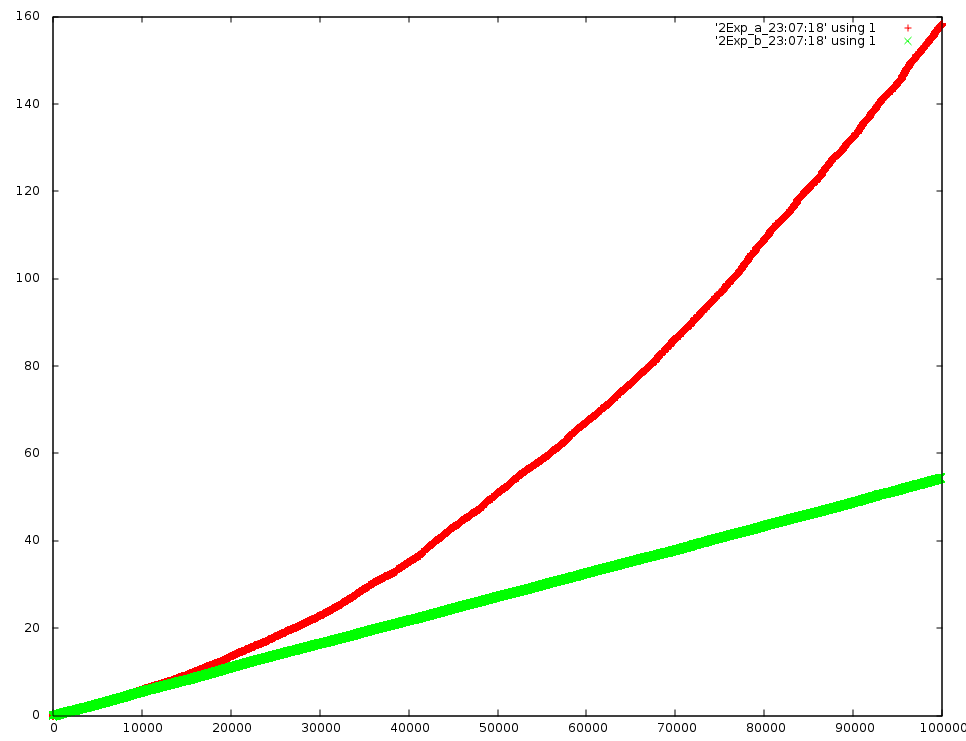
\includegraphics[width=12cm]{img/relative}
\end{figure}

\begin{figure}[h!]
  \centering
  \caption{Accumulated relative error for 4 000 highscore updates. Red line is the old algorithm, green line is the algorithm with dynamic bucket-table}
  \label{fig:relerror4000}
  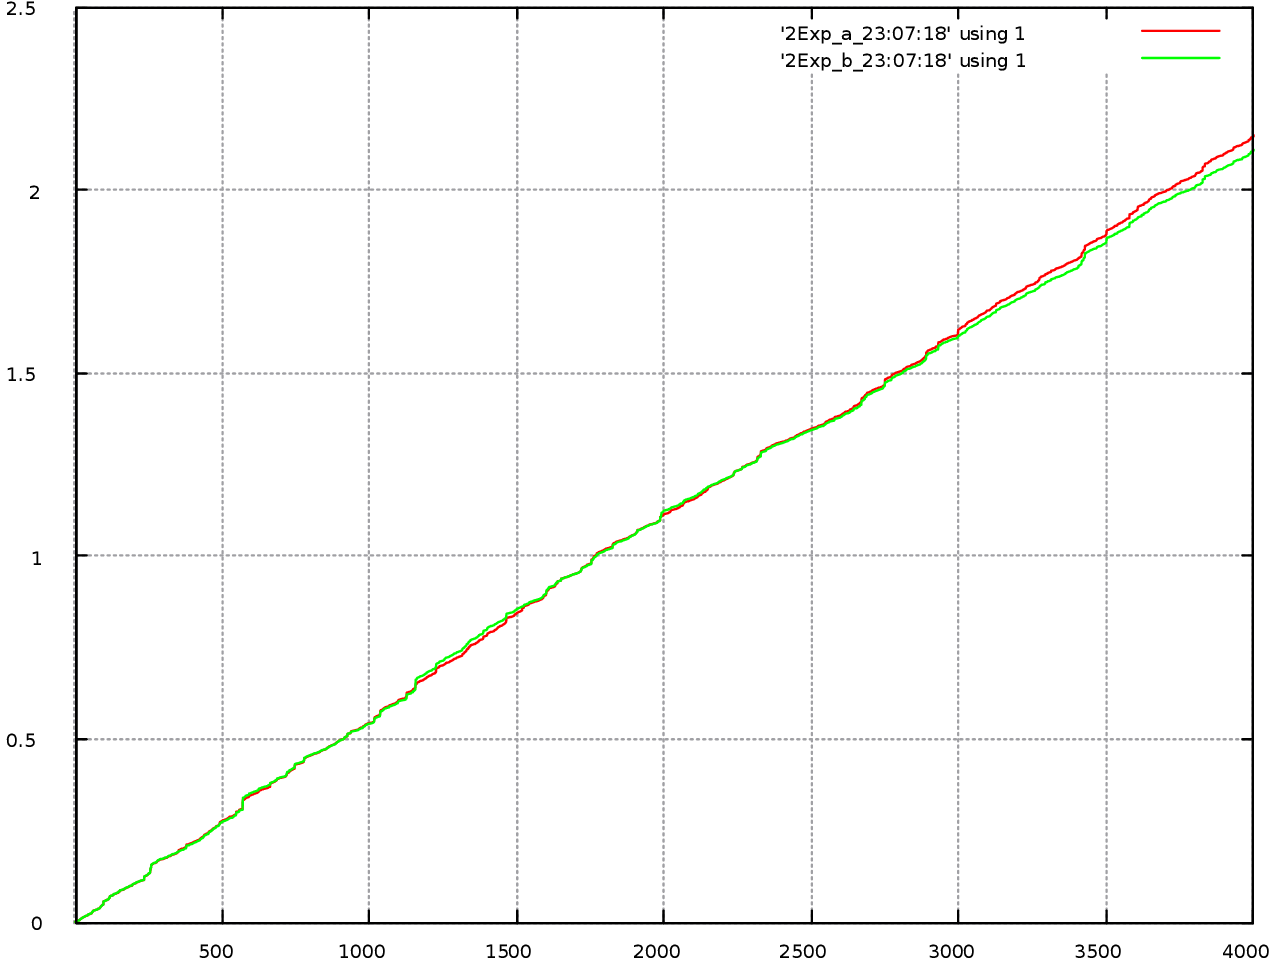
\includegraphics[width=12cm]{img/acc-rel-error}
\end{figure}

\section{Execution time}

Execution time for ranking 4000 highscores with the current implementation is 25 687 ms and 30 180 ms. 

Building a bucket-table for 100 000 highscores takes 10 205 ms in average. 

\begin{figure}[h!]
  \centering
  \caption{Execution time for 4 000 highscore updates. Red line is the old algorithm, green line is the algorithm with dynamic bucket-table}
  \label{fig:relerror}
  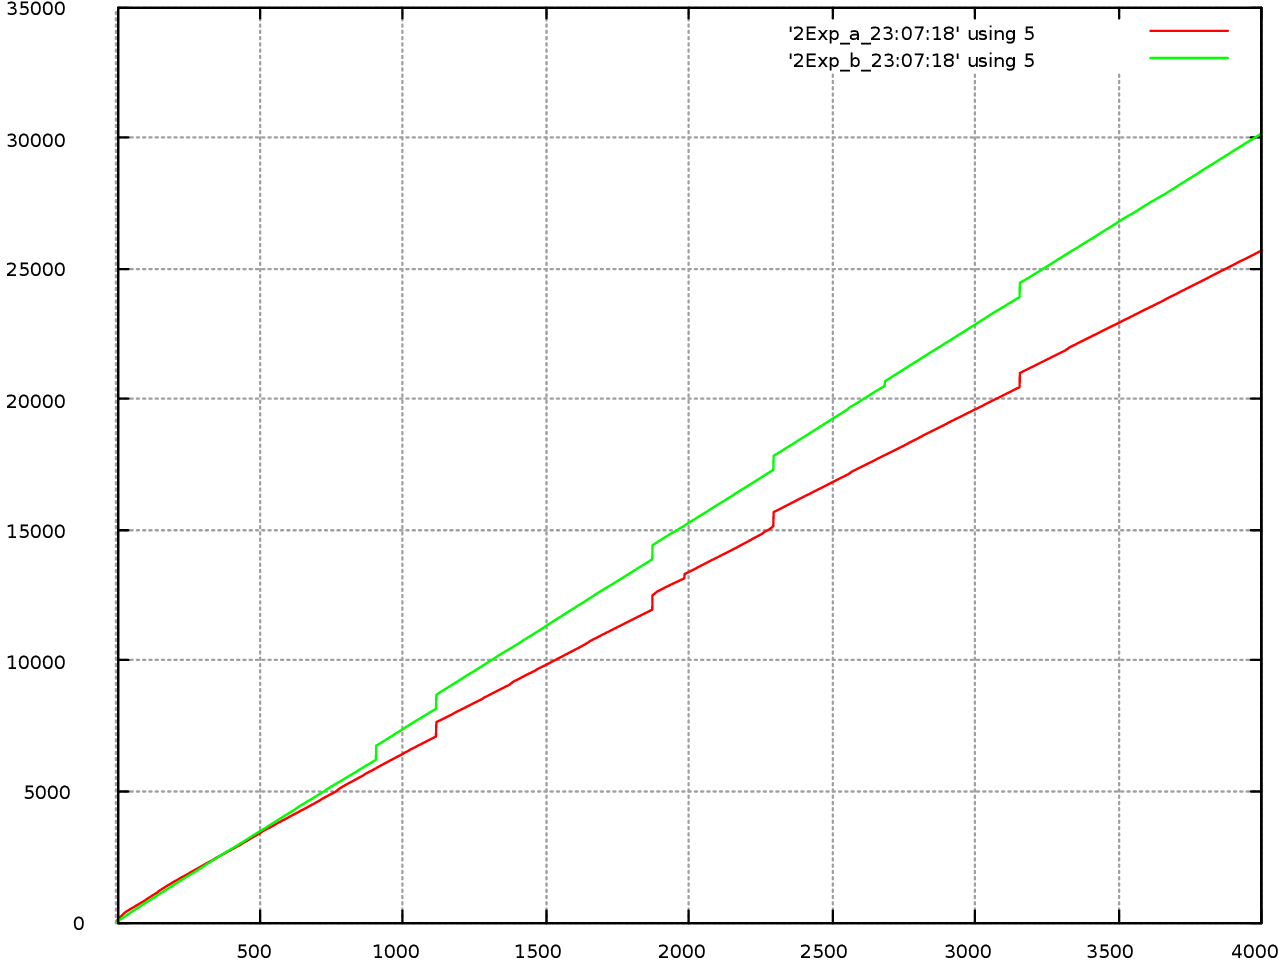
\includegraphics[width=12cm]{img/exec-time} 
\end{figure}

\section{Interim results}

Since the relative error seems to be in control with the improved algorithm for as many as 100 000 rankings we can assume that it would produce good enough rankings for five hours.

The execution time with the current implementation for five hours would then be $5 \times 6 \times 10 205 ms + \frac{100 000}{4000} \times 25 687 = 948 325 ms$

For the improved algorithm, $10 205 ms + \frac{100 000}{4000} \times 30 180 = 764705 ms$.
